\documentclass[a4paper, 12pt]{article}

%Oтступы
\usepackage[left=2cm,right=2cm,top=2cm,bottom=2cm,bindingoffset=0cm]{geometry}

%Русский язык
\usepackage[T2A]{fontenc} %кодировка
\usepackage[utf8]{inputenc} %кодировка исходного кода
\usepackage[english,russian]{babel} %локализация и переносы

%Вставка картинок
\usepackage{wrapfig}
\usepackage{graphicx}
\graphicspath{{pictures/}}
\DeclareGraphicsExtensions{.pdf,.png,.jpg}

%оглавление
\usepackage{titlesec}
\titlespacing{\chapter}{0pt}{-30pt}{14pt}
\titlespacing{\section}{\parindent}{5mm}{5mm}
\titlespacing{\subsection}{\parindent}{5mm}{5mm}
\usepackage{setspace}

%Графики
\usepackage{multirow}
%usepackage{pgfplots}
%pgfplotsset{compat=1.9}

%Математика
\usepackage{mathrsfs}
\usepackage{amsmath, amsfonts, amssymb, amsthm, mathtools}
%DeclareMathAlphabet{\mathcalligra}{T1}{calligra}{m}{n}

\usepackage{multicol}

\usepackage[usenames,dvipsnames,svgnames,table]{xcolor}
\usepackage{lettrine} % To make a Drop Cap
\usepackage{yfonts} % to make a fancy Gothic drop caps.

\usepackage{lastpage} 

\newcommand{\angstrom}{\mbox{\normalfont\AA}}


\begin{document} 
		\begin{titlepage}
		\hfill
		\vfill
			\begin{center}
				\vspace{13ex}
				\textbf{Лабораторные работы №2.2 и №2.3}
				\vspace{1ex}\\
				на тему:\\	\textbf{\Large{<<Изучение спектров атомов водорода и йода>>}}
				
				\vspace{30ex}
				\begin{flushright}
					\noindent
					\textit{Работу выполнил:}
					
					\textit{Олейник Роман}
					
				\end{flushright}
				\vfill
			\end{center}
		\end{titlepage}
		
		\newpage
\section*{Аннотация}
Целями данной работы являются исследование сериальных закономерностей в оптическом спектре водорода и исследование спектра поглощения паров йода в видимой области.
\section*{Теоретические сведения: спектр водорода}
Атом водорода является простейшей квантовой системой, для которой уравнение Шрёдингера может быть решено точно. Это также верно для водородноподобных атомов, то есть атомов с одним электроном на внешней оболочке. Из решения уравнения Шрёдингера следует, что внешний электрон в таких атомах обладает дискретным энергетическим спектром:  
	\begin{equation}
			E_n = - \frac{m_e (Z e^2)^2}{2\hbar^2}\frac{1}{n^2},
	\end{equation}
где $n$ есть номер энергетического уровня, $Z$ есть зарядовое число ядра рассматриваемого атома, которое в случае атома водорода равно 1.\\
При переходе электрона с $n$-го на $m$-й уровень излучается фотон с энергией
	\begin{equation}
		E_\gamma = E_n - E_m = \frac{m_ee^2}{2\hbar^2}Z^2\left(\frac{1}{m^2} - \frac{1}{n^2}\right).
	\end{equation}
	Длина волны  соответствующего излучения $\lambda_{n,m}$ связана с номерами уровней следующим соотношением:
	\begin{equation}
	\lambda_{n,m}^{-1} =\frac{m_ee^2}{4\pi\hbar^3c}Z^2\left(\frac{1}{m^2}-\frac{1}{n^2}\right) = \text{Ry} Z^2 \left(\frac{1}{m^2}-\frac{1}{n^2}\right),
	\end{equation}
	где $\text{Ry} = \frac{m_ee^2}{4\pi\hbar^3c}$ есть постоянная Ридберга.\\ 
	В данной работе будет исследоваться серия Бальмера атома водорода, в которой электроны совершают переходы с некоторого уровня $n$ на уровень $m = 2$.
\section*{Теоретические сведения: спектр йода}
В первом приближении энергия молекулы может быть представлена в виде:
\begin{equation}
E=E_e+E_o+E_r,
\end{equation}
где $E_e$ есть энергия электронных уровней, $E_o$ есть энергия колебательньных уровней, $E_r$ есть энергия вращательных уровней.\\
В данной работе рассматриваются оптические переходы, то есть переходы, связанные с излучением фотонов в видимом диапазоне длин волн. Они соответсвтуют переходам между различными электронными состояниями. При этом также происходят изменения вращательного и колебательного состояний, однако в реальности ввиду малости характерных энергий вращательные переходы ненаблюдаемы.\\
Более конкретно, изучаются переходы из колебательного состояния с номером $n_1$ освновного электронного уровня с энергией $E_1$ в колебательное состояние с номером $n_2$ на электронный уровень с энергией $E_2$. Энергия таких переходов описывается формулой:
\begin{equation}
h \nu_{n_1,n_2}=(E_2-E_1)+h\nu_2(n_2+\dfrac{1}{2})-h \nu_1(n_1+\dfrac{1}{2}),
\end{equation}
где $\nu_1$ и $\nu_2$ суть энергии колебательных квантов на электронных уровнях с энергиями $E_1$ и $E_2$.\\
При достаточно больших квантовых числах $n_1$ и $n_2$ колебательные уровни переходят в непрерывный спектр, что соответствует диссоциации молекулы. Наименьшая энергия, которую нужно сообщить молекуле в нижайшем колебательном состоянии, чтобы она диссоциировала, называется энергией диссоциации.\\
В данной работе определяются энергии диссоциации на первых двух электронных уровнях.
\section*{Обработка результатов}
Во-первых, проградуируем спектрометр, для чего используем спектры неоновой и ртутной лампы, длины волн спектральных линий которых известны. Приведём соответствующую таблицу.\\
\begin{figure}[h!]
\center{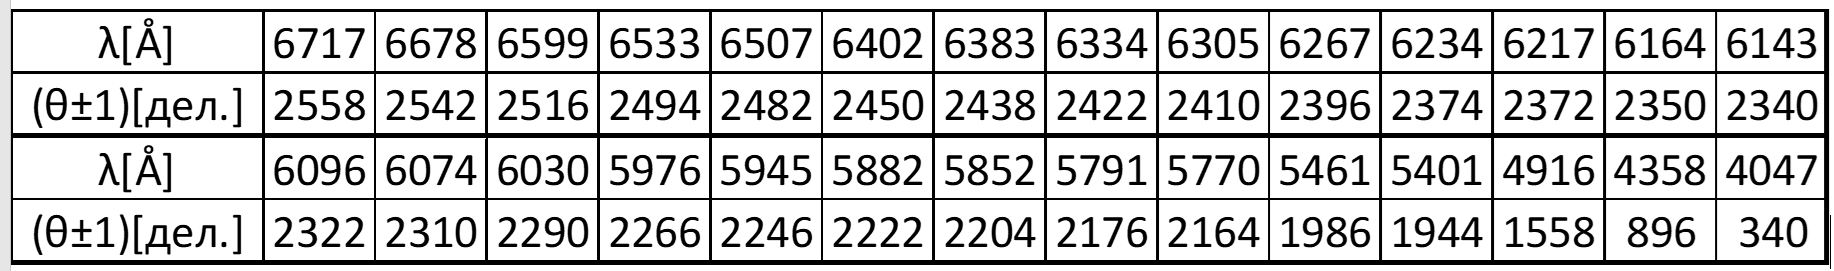
\includegraphics[width=15 cm]{Table}}
\end{figure}\\
Построим также градуировочный график.\\
\begin{figure}[h!]
\center{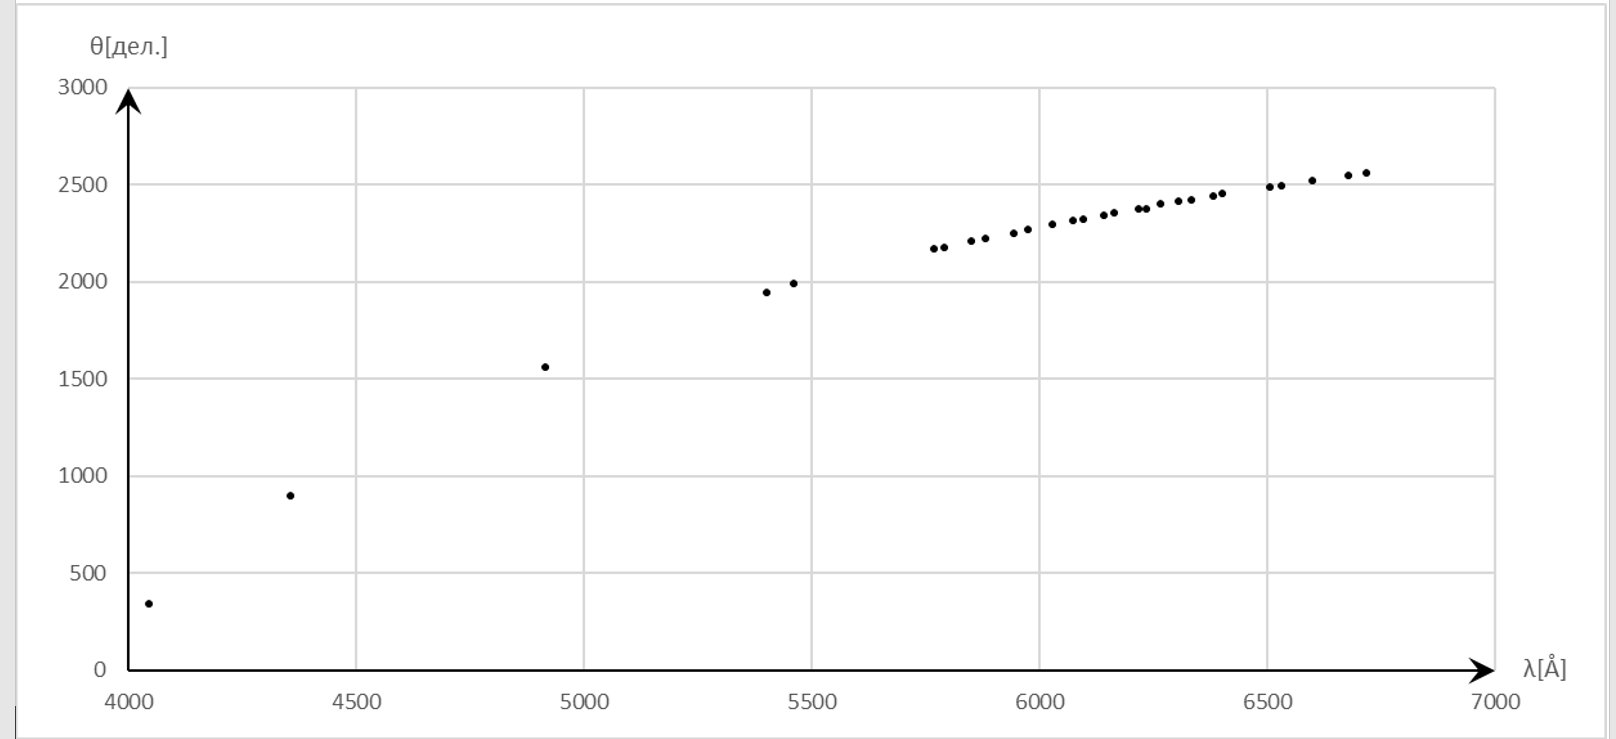
\includegraphics[width=15 cm]{Graph}}
\end{figure}\\
Для интерполяции данного графика на все промежуточные значения используем формулу Гартмана:
\begin{equation}
\lambda=\lambda_0+\dfrac{C_0}{\theta-\theta_0},
\end{equation}
где $\lambda_0, C_0,\theta_0$ суть параметры, определяемые по трём ближайшим точкам графика.\\
Измерим положения трёх линий водорода из серии Бальмера --- $H_{\alpha}, H_{\beta}, H_{\gamma}$. Линию $H_{\delta}$ пронаблюдать не удалось ввиду её слабой интенсивности.\\
Получили соответствующие показания спектрометра: $H_{\alpha}$ --- $2500\pm 1$, $H_{\beta}$ --- $1508 \pm 1$, $H_{\gamma}$ --- $874 \pm 1$.\\
С учётом градуировки спектрометра получаем следующие длины волн: $H_{\alpha}$ --- $656 \pm 2$ нм, $H_{\beta}$ --- $487 \pm 2$ нм, $H_{\gamma}$ --- $434 \pm 2$ нм.\\
Для каждой линии определим константу Ридберга по формуле (3), учитывая, что $m=2$, $Z=1$, а также, что для линии $H_{\alpha}$ --- $n=3$, для линии $H_{\beta}$ --- $n=4$,для линии $H_{\gamma}$ --- $n=5$.\\
Получаем следующие значения константы Ридберга: $\text{Ry}_{\alpha}=0.0110 \pm 0.0001$ нм$^{-1}$, $\text{Ry}_{\beta}=0.0109 \pm 0.0001$ нм$^{-1}$, $\text{Ry}_{\gamma}=0.0109 \pm 0.0001$ нм$^{-1}$.\\
По МНК определяем наилучшее значение константы Ридберга, а также его погрешность: $\text{Ry}_E=(0.0109\pm 0.0002)$ нм$^{-1}$.\\
Полученное значение в пределах погрешности совпадает с табличным значением: $\text{Ry}_T=0.01097$ нм$^{-1}$.\\
Запишем показания спектрометра для следующих переходов в молекуле йода: $\theta_{1,0}$ --- переход из первого колебательного уровня основного состояния в нулевой колебательный уровень возбуждённого состояния,  $\theta_{1,5}$ --- переход из первого колебательного уровня основного состояния в пятый колебательный уровень возбуждённого состояния, $\theta_{g}$ --- переход из нулевого колебательного уровня основного состояния в область непрерывного спектра возбуждённого состояния.\\
Получаем следующие данные: $\theta_{1,0}=2344 \pm 1$, $\theta_{1,5}=2242 \pm 1$, $\theta_g=1850 \pm 1$. Отсюда находим соответствующие длины волн: $\lambda_{1,0}=615 \pm 2$ нм, $\lambda_{1,5}=594 \pm 2$ нм, $\lambda_g=522 \pm 2$ нм.\\
Определим энергию колебательного кванта возбуждённого состояния молекулы по формуле: $h \nu_2=\dfrac{h\nu_{1,5}-h \nu_{0,5}}{5}$. Проделав вычисления, получаем, что $h\nu_2=0.014\pm 0.002$ эВ.\\
Вычислим энергию электронного перехода $\Delta E=E_2-E_1$, энергию диссоциации $D_1$ в основном состоянии и энергию диссоциации $D_2$ в возбуждённом состоянии, если известно, что энергия колебательного кванта основного состояния равна $h\nu_1=0,027$ эВ, а энергия возбуждения, то есть энергия перехода атома из области непрерывного спектра основного состояния в область непрерывного спектра возбуждённого состояния, равна $E_A=0.94$ эВ.\\
Имеем систему уравнений:
\begin{equation}
D_1+E_A=h \nu_g,
\end{equation}
\begin{equation}
h\nu_g=D_2+\Delta E,
\end{equation}
\begin{equation}
h\nu_{1,0}=\Delta E+h\nu_2-\dfrac{3}{2}h\nu_1,
\end{equation}
\begin{equation}
h\nu_{1,5}=\Delta E+\dfrac{11}{2}h\nu_2-\dfrac{3}{2}h\nu_1.
\end{equation}
Из неё находим все необходимые значения: $\Delta E=2.050\pm 0.002$ эВ, $D_1=1.436\pm 0.002$ эВ, $D_2=0.326 \pm 0.002$ эВ.
\section*{Вывод}
В работе исследовались сериальные закономерности в оптическом спектре водорода и спектр поглощения паров йода в видимой области.\\
С помощью информации о спектральных линиях неона и ртути проградуирован спектрометр. Построен соответствующий график.\\
Получены длины волн линий $H_{\alpha}$, $H_{\beta}$ и $H_{\gamma}$ серии Бальмера, вычислена постоянная Ридберга. В рамках погрешности данные совпали с табличными.\\
Получены длины волн, соответствующие некоторым электронно-колебательным переходам из основного состояния в возбуждённое. Вычислены энергия колебательного кванта возбуждённого состояния молекулы, энергия электронного перехода, энергии диссоциации молекулы в основном и в возбуждённом состояниях.\\
Все поставленные задачи выполнены, работа завершена успешно.
\end{document}
